
\documentclass[letterpaper, reqno,11pt]{article}
\usepackage[margin=1.0in]{geometry}
\usepackage{color,latexsym,amsmath,amssymb}
\usepackage{fancyhdr}
\usepackage{amsthm}
\usepackage{mathtools}
\usepackage{tikz}
\usepackage{float}
\usepackage{centernot}
\usepackage{subcaption}
\usepackage{extarrows}
\usetikzlibrary{hobby}
\usepackage{pgfplots}

\newcommand{\RR}{\mathbb{R}}
\newcommand{\CC}{\mathbb{C}}
\newcommand{\ZZ}{\mathbb{Z}}
\newcommand{\QQ}{\mathbb{Q}}
\newcommand{\NN}{\mathbb{N}}
\DeclareMathOperator{\card}{card}
\DeclareMathOperator{\Binomial}{Binomial}
\pagestyle{fancy}
\lhead{Math 321 Lecture 5}
\rhead{Yuchong Pan}
\begin{document}
\pagenumbering{arabic}
\title{Math 321 Lecture 5}
\author{Yuchong Pan}
\date{January 11, 2019}
\newtheorem{thm}{Theorem}
\newtheorem{defn}{Definition}
\newtheorem{exs}{Exercise}
\newtheorem{remark}{Remark}
\newtheorem{claim}{Claim}
\newtheorem{cor}{Corollary}
\maketitle
%

\section{Applications of Pointwise and Uniform Convergence}

\subsection{Weierstrass Approximation Theorem (Take 1)}

\begin{thm}[Weierstrass approximation theorem] \label{thm:1}
  \normalfont Let $a, b \in \RR, a < b$. Every $f \in C[a, b]$ can be uniformly approximated by polynomials; i.e., given any $f : [a, b] \xrightarrow{\text{continuous}} \RR \text{ or } \CC$, there exists a sequence $\{ p_n : n \geq 1 \} \subseteq \mathcal P[a, b]$, where $\mathcal P[a, b]$ is the space of polynomials on $[a, b]$ with coefficients in $\RR$ or $\CC$, such that $p_n \xrightarrow{n \to \infty} f$ uniformly on $[a, b]$.
\end{thm}

\begin{cor}
  \normalfont $C[a, b]$ is {\bf separable}; i.e., it has a countable dense subset.
\end{cor}

\begin{proof}
  $\mathcal P[a, b]$, i.e., the space of real/complex polynomials on $[a, b]$, is dense in $C[a, b]$ by Weierstrass approximation theorem, but not countable.

  Define $\mathcal P^*[a, b] = \bigcup_{n = 0}^\infty \mathcal P_n^* [a,b]$, where
  \begin{multline*}
    \mathcal P_n^*[a, b] = \left\{ p : [a, b] \to \RR \text{ (or $\CC$)} ; p(x) = c_0 + c_1 x + c_2 x^2 + \ldots + c_n x^n \right. \\
    \qquad \left. \text{ for some } (c_0, c_1, \ldots, c_n) \in \QQ^{n + 1} \text{ (or $(\QQ + i\QQ)^{n + 1}$)} \right\}
  \end{multline*}
  i.e., $\mathcal P_n^*[a, b]$ contains polynomials on $[a, b]$ of degree $\leq n$.
  
  ~
  
  \noindent {\bf Need to show:}
  \begin{enumerate}
  \item $\mathcal P^*$ is countable.

    It suffices to show each $\mathcal P_n^*$ is countable. Fix any $n \geq 1$, and define $\varphi : \QQ^{n + 1} \to \mathcal P_n^*$ by
    $$ \varphi(c_0, c_1, \ldots, c_n) = \sum_{i = 0}^n c_i x^i. $$
    Then $\varphi$ is a bijection. Thus, $\card\left(\mathcal P_n^*\right) = \card\left(\QQ^{n + 1}\right)$, where $\QQ^{n + 1}$ is countable.
  \item $\mathcal P^*$ is dense.
    
    \noindent {\bf Know:} $\mathcal P^* \subsetneq \mathcal P \overset{\text{\small dense}}{\subsetneq} C[a, b]$.

    It suffices to show that $\mathcal P^*$ is dense in $\mathcal P$ (show why).

    Start with any $f \in \mathcal P$; i.e., $f(x) = \sum_{i = 0}^n \alpha_i x^i, \alpha_i \in \RR \text{ or } \CC$. Since $\QQ$ (respectively, $\QQ + i\QQ$) is dense in $\RR$ (respectively, $\CC$), we can find sequences of rationals $\left\{ c_i^{(k)} : k \geq 1 \right\}, 0 \leq i \leq n$ such that $c_i^{(k)} \xrightarrow{k \to \infty}\alpha_i$ for all $0 \leq i \leq n$.

    Define $p_k(x) = \sum_{i = 0}^n c_i^{(k)} x^i \in \mathcal P^*$, for all $k \geq 1$. Then
    \begin{align*}
      \lVert p_k - f \rVert_\infty &= \sup_{x \in [a, b]} |p_k(x) - f(x)| \\
      &= \sup_{x \in [a, b]} \left|\sum_{i = 0}^n \left(c_i^{(k)} - \alpha_i\right) x^i\right| \\
      &\leq \sup_{x \in [a, b]} \sum_{i = 0}^n \left|c_i^{(k)} - \alpha_i\right| |x|^i \\
      &\leq M \sum_{i = 0}^n \left|c_i^{(k)} - \alpha_i\right|,
    \end{align*}
    where $M = \max\left\{ |x|^i : x \in [a, b], 0 \leq i \leq n \right\} < \infty$. Since $\left|c_i^{(k)} - \alpha_i\right| \to 0$ as $k \to \infty$, then $\lVert p_k - f\rVert_\infty \to 0$ as $k \to \infty$.
  \end{enumerate}
\end{proof}

\begin{proof}[Proof of Theorem \ref{thm:1} (Bernstein)]
  \renewcommand{\qedsymbol}{}
  Start with $f \in C[0, 1]$. Note that it suffices to consider $C[0, 1]$ because $[a, b] \xrightarrow[\text{linear}]{\text{bijection}} [0, 1]$ by $x \mapsto \frac{x - a}{b - a}$.

  Define $p_n(f)(x) = \sum_{k = 0}^\infty f\left(\frac{k}{n}\right)\underbrace{\binom{n}{k} x^k (1 - x)^{n - k}}_\text{binomial probabilities}$. Then $p_n(f)$ is a polynomial of degree $\leq n$. If we regard $\binom{n}{k} x^k (1 - x)^{n - k}$ as binomial probabilities, then $p_n(f)(x) = \mathbb E f\left(\frac{X}{n}\right), X \sim \Binomial(n, x)$.

  \begin{figure}[H]
    \centering
    \renewcommand{\arraystretch}{2}
    \begin{tabular}{c|c}
      $f\left(\frac{i}{n}\right)$ & $\mathbb P(X = i)$ \\
      \hline
      $f\left(\frac{0}{n}\right)$ & $\binom{n}{0} x^0 (1 - x)^{n - 0}$ \\
      \hline
      $f\left(\frac{1}{n}\right)$ & $\binom{n}{1} x^1 (1 - x)^{n - 1}$ \\
      \hline
      $\vdots$ & $\vdots$ \\
      \hline
      $f\left(\frac{k}{n}\right)$ & $\binom{n}{k} x^k (1 - x)^{n - k}$
    \end{tabular}
    \renewcommand{\arraystretch}{1}
  \end{figure}

  Fix $\epsilon > 0$. We want to find $N \geq 1$ such that for all $n \geq N$, $\lVert p_n - f\rVert_\infty < \epsilon$. Note that

  \begin{align*}
    \sup_{x \in [0, 1]} |p_n(f)(x) - f(x)| &= \sup_{x \in [0, 1]} \left|\sum_{k = 0}^n f\left(\frac{k}{n}\right)\binom{n}{k} x^k (1 - x)^{n - k} - f(x) \cdot 1\right| \\
    &= \sup_{x \in [0, 1]} \left|\sum_{k = 0}^n f\left(\frac{k}{n}\right)\binom{n}{k} x^k (1 - x)^{n - k} - f(x) \cdot \sum_{k = 0}^n \binom{n}{k} x^k (1 - x)^{n - k}\right| \\
    &= \sup_{x \in [0, 1]} \left|\sum_{k = 0}^n \left(f\left(\frac{k}{n}\right) - f(x)\right) \binom{n}{k} x^k (1 - x)^{n - k}\right|.
  \end{align*}
  By the {\bf uniform} convergence of $f$, there exists $\delta > 0$ such that $|f(x) - f(y)| < \frac{\epsilon}{2}$ whenever $|x - y| < \epsilon$. Then,
  \begin{multline*}
    \sup_{x \in [0, 1]} |p_n(f)(x) - f(x)| \leq \sup_{x \in [0, 1]} \left(\underbrace{\sum_{\substack{k = 0 \\ \left|\frac{k}{n} - x\right| < \delta}}^n \overbrace{\left|f\left(\frac{n}{k}\right) - f(x)\right|}^{< \frac{\epsilon}{2}} \binom{n}{k} x^k (1 - x)^{n - k}}_\text{I} \right. \\
    + \left. \underbrace{\sum_{\substack{k = 0 \\ \left|\frac{k}{n} - x\right| \geq \delta}}^n \left|f\left(\frac{n}{k}\right) - f(x)\right| \binom{n}{k} x^k (1 - x)^{n - k}}_\text{II}\right).
  \end{multline*}

  Note that $\text{I} < \frac{\epsilon}{2}$ because $\sum_{\left|\frac{k}{n} - x\right| < \delta} \binom{n}{k} x^k (1 - x)^{n - k} \leq 1$.

  \begin{figure}[H]
    \centering
    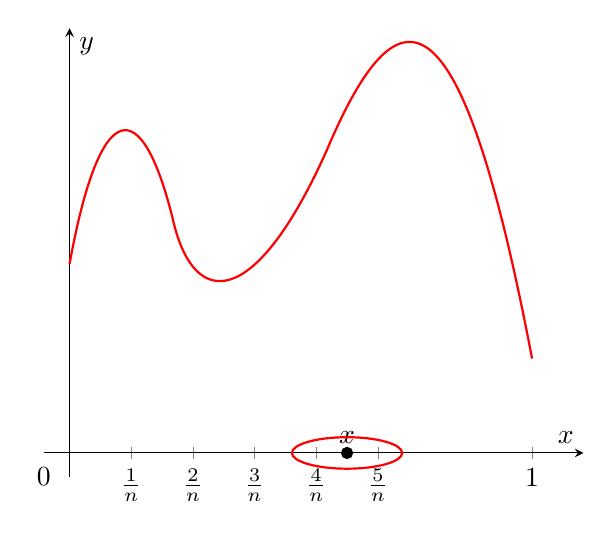
\begin{tikzpicture}
      \begin{axis}[
          xmin=-0.25,
          xmax=5,
          ymin=-0.25,
          ymax=4.5,
          xtick={0.6, 1.2, 1.8, 2.4, 3, 4.5},
          xticklabels={$\frac{1}{n}$, $\frac{2}{n}$, $\frac{3}{n}$,$\frac{4}{n}$, $\frac{5}{n}$, $1$},
          ymajorticks=false,
          xlabel={$x$},  
          ylabel={$y$},
          axis lines=middle]
        \draw[fill=black] (axis cs:2.7, 0) circle (2pt) node[above] {$x$};
        \draw[thick, red] (axis cs:2.7, 0) ellipse (0.7cm and 0.2cm);
        \draw[thick, red] (axis cs:0, 2) .. controls (axis cs:0.3, 3.8) and (axis cs:0.7, 3.8) .. (axis cs:1, 2.5) .. controls (axis cs:1.2, 1.5)  and (axis cs:1.8, 1.5) .. (axis cs:2.5, 3.2) .. controls (axis cs:3.2, 5) and (axis cs: 3.8, 5) .. (axis cs:4.5, 1);
      \end{axis}
      \node at (0, 0) {$0$};
    \end{tikzpicture}
  \end{figure}

  ~

  (Proof unfinished.)
\end{proof}

\end{document}
